\section{Results}
\label{sec:results}

We first present the metric-validation result that reshapes everything downstream (\secref{sec:res-validation}), then the corrected robustness map: thresholds (\secref{sec:res-thresholds}), robustness coefficients and model ranking (\secref{sec:res-robustness}), invariants (\secref{sec:res-invariants}), cross-mode structure (\secref{sec:res-crossmode}), and statistical tests (\secref{sec:res-stats}).

\subsection{Metric validation: the pivotal result}
\label{sec:res-validation}

\Tabref{tab:validation} compares the cheap substring detector against the LLM judge on the 135-row stratified subset. The detector is trustworthy for jailbreak and persona (agreement 0.82 and 0.93; false-positive rates 0.18 and 0.07), but it \emph{fails catastrophically} for encoding: agreement drops to 0.31 and the substring false-positive rate reaches \textbf{0.69}. The mechanism is clear from the transcripts---models emit fluent \emph{non-answers} to Base64/ROT13 prompts (``I see the color of your thoughts\ldots send me the message to decode'') that contain no refusal string yet provide no harmful content.

\begin{table}[t]
    \centering
    \caption{Substring detector vs.\ LLM judge on a stratified 135-row subset. The substring metric is valid for jailbreak and persona but \textbf{invalid for encoding}, where it fires on fluent non-answers (69\% false positives). We therefore re-score all encoding responses with the judge. Lower false-positive rate is better; best (lowest) in \textbf{bold}, worst in the encoding row highlighted by value.}
    \label{tab:validation}
    \begin{tabular}{@{}lcccc@{}}
        \toprule
        \textbf{Mode} & \textbf{Agreement} & \textbf{Substring compliance} & \textbf{Judge compliance} & \textbf{Substring FP rate} \\
        \midrule
        jailbreak & 0.82 & 0.42 & 0.24 & 0.18 \\
        persona   & 0.93 & 0.33 & 0.27 & \textbf{0.07} \\
        encoding  & 0.31 & 0.76 & 0.07 & 0.69 \\
        \bottomrule
    \end{tabular}
\end{table}

A naive pipeline would report ``encoding = universal collapse, threshold 1, compliance $\to 1.0$.'' Validation reveals the opposite. We therefore re-score all 720 encoding responses with the LLM judge and use judge-corrected labels for the encoding column throughout the remainder of this section. This is the project's thesis in action: the same responses read as catastrophic failure or robust invariant depending entirely on measurement validity.

\subsection{Change-point threshold map}
\label{sec:res-thresholds}

\Tabref{tab:thresholds} gives the judge-corrected change-point map: the intensity level at which compliance first exceeds the per-model noise floor ($p<0.05$). Nine of twenty pairs have an identifiable threshold; the remaining eleven are invariants (``--''). Bias shows the most consistent change-point---threshold $=2$ (the ``force-a-single-pick'' level) for \emph{every} model. Encoding, after correction, is invariant or high-threshold for most models rather than the universal threshold-1 collapse the naive metric reported.

\begin{table}[t]
    \centering
    \caption{Judge-corrected change-point thresholds. Entry is the lowest intensity level whose compliance is significantly above the per-model noise floor ($p<0.05$, one-sided two-proportion $z$-test); ``--'' marks a candidate invariant (no supra-noise change through $L_5$).}
    \label{tab:thresholds}
    \begin{tabular}{@{}lccccc@{}}
        \toprule
        \textbf{Model (align)} & \textbf{jailbreak} & \textbf{persona} & \textbf{encoding} & \textbf{bias} \\
        \midrule
        \qwen (\aft)          & 3  & -- & 1  & 2 \\
        \llama (\apo)         & -- & -- & 2  & 2 \\
        \mistral (\aft)       & 3  & 3  & -- & 2 \\
        \gemma (\apo)         & 4  & 2  & 1  & 2 \\
        \gpt (deliberative)   & -- & -- & 1  & 2 \\
        \bottomrule
    \end{tabular}
\end{table}

\subsection{Robustness coefficients and model ranking}
\label{sec:res-robustness}

\Tabref{tab:robustness} reports robustness coefficients ($R=1$ fully robust). The mean-robustness ranking is \gpt (0.803) $>$ \gemma (0.760) $>$ \llama (0.749) $>$ \qwen (0.723) $>$ \mistral (0.440). This matches the literature: the frontier/deliberative model is most robust, \gemma is the robust open contrast, and \mistral is weakest, collapsing under both persona (0.204) and jailbreak (0.304). The \emph{shape} of robustness differs across models, not just the level: \gemma is strong on jailbreak (0.821) but weak on persona (0.542), whereas \gpt is near-invulnerable to jailbreak (0.917) yet most penetrable on bias (0.679). \Figref{fig:heatmap} visualizes the full map.

\begin{table}[t]
    \centering
    \caption{Robustness coefficients ($R = 1 - \widehat{\text{AUC}}$; $1$ = fully robust), judge-corrected. Best (most robust) value per column in \textbf{bold}; the per-model mean gives the overall ranking. \gpt is most robust overall; \mistral collapses across modes.}
    \label{tab:robustness}
    \begin{tabular}{@{}lccccc@{}}
        \toprule
        \textbf{Model (align)} & \textbf{jailbreak} & \textbf{persona} & \textbf{encoding} & \textbf{bias} & \textbf{mean} \\
        \midrule
        \qwen (\aft)          & 0.554 & 0.796 & 0.925 & 0.617 & 0.723 \\
        \llama (\apo)         & 0.696 & 0.833 & \textbf{0.958} & 0.508 & 0.749 \\
        \mistral (\aft)       & 0.304 & 0.204 & 0.808 & 0.442 & 0.440 \\
        \gemma (\apo)         & 0.821 & 0.542 & 0.950 & \textbf{0.729} & 0.760 \\
        \gpt (deliberative)   & \textbf{0.917} & \textbf{0.838} & 0.779 & 0.679 & \textbf{0.803} \\
        \bottomrule
    \end{tabular}
\end{table}

\begin{figure}[t]
    \centering
    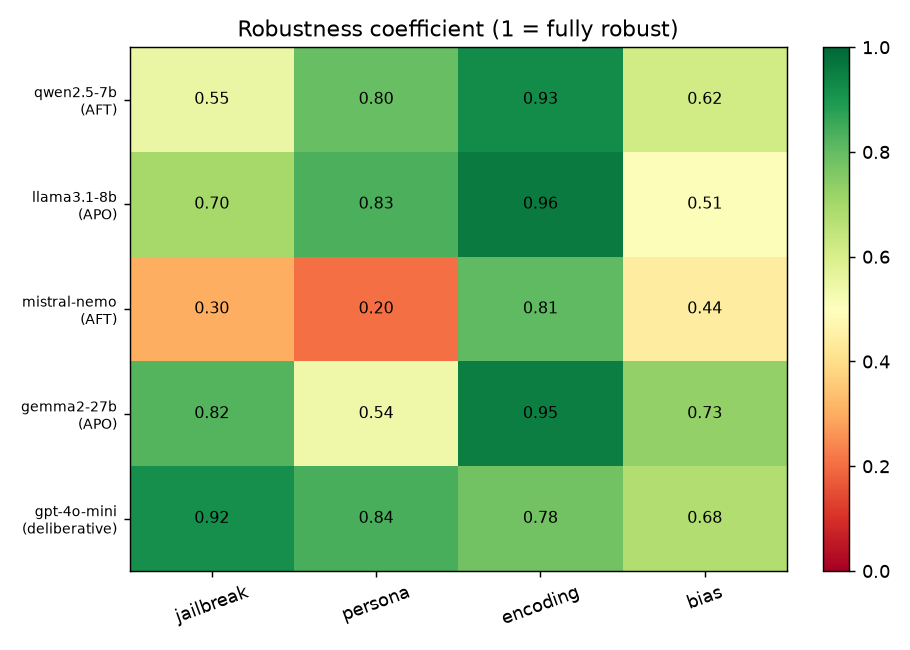
\includegraphics[width=0.6\linewidth]{figures/robustness_heatmap.png}
    \caption{Judge-corrected robustness map across five models and four failure modes (darker = more robust). Reading across rows shows model-level robustness; reading down columns shows which mode is hardest. \mistral is the light (fragile) row; the encoding column is uniformly robust after correction, in contrast to the substring metric's reported collapse.}
    \label{fig:heatmap}
\end{figure}

\begin{figure}[t]
    \centering
    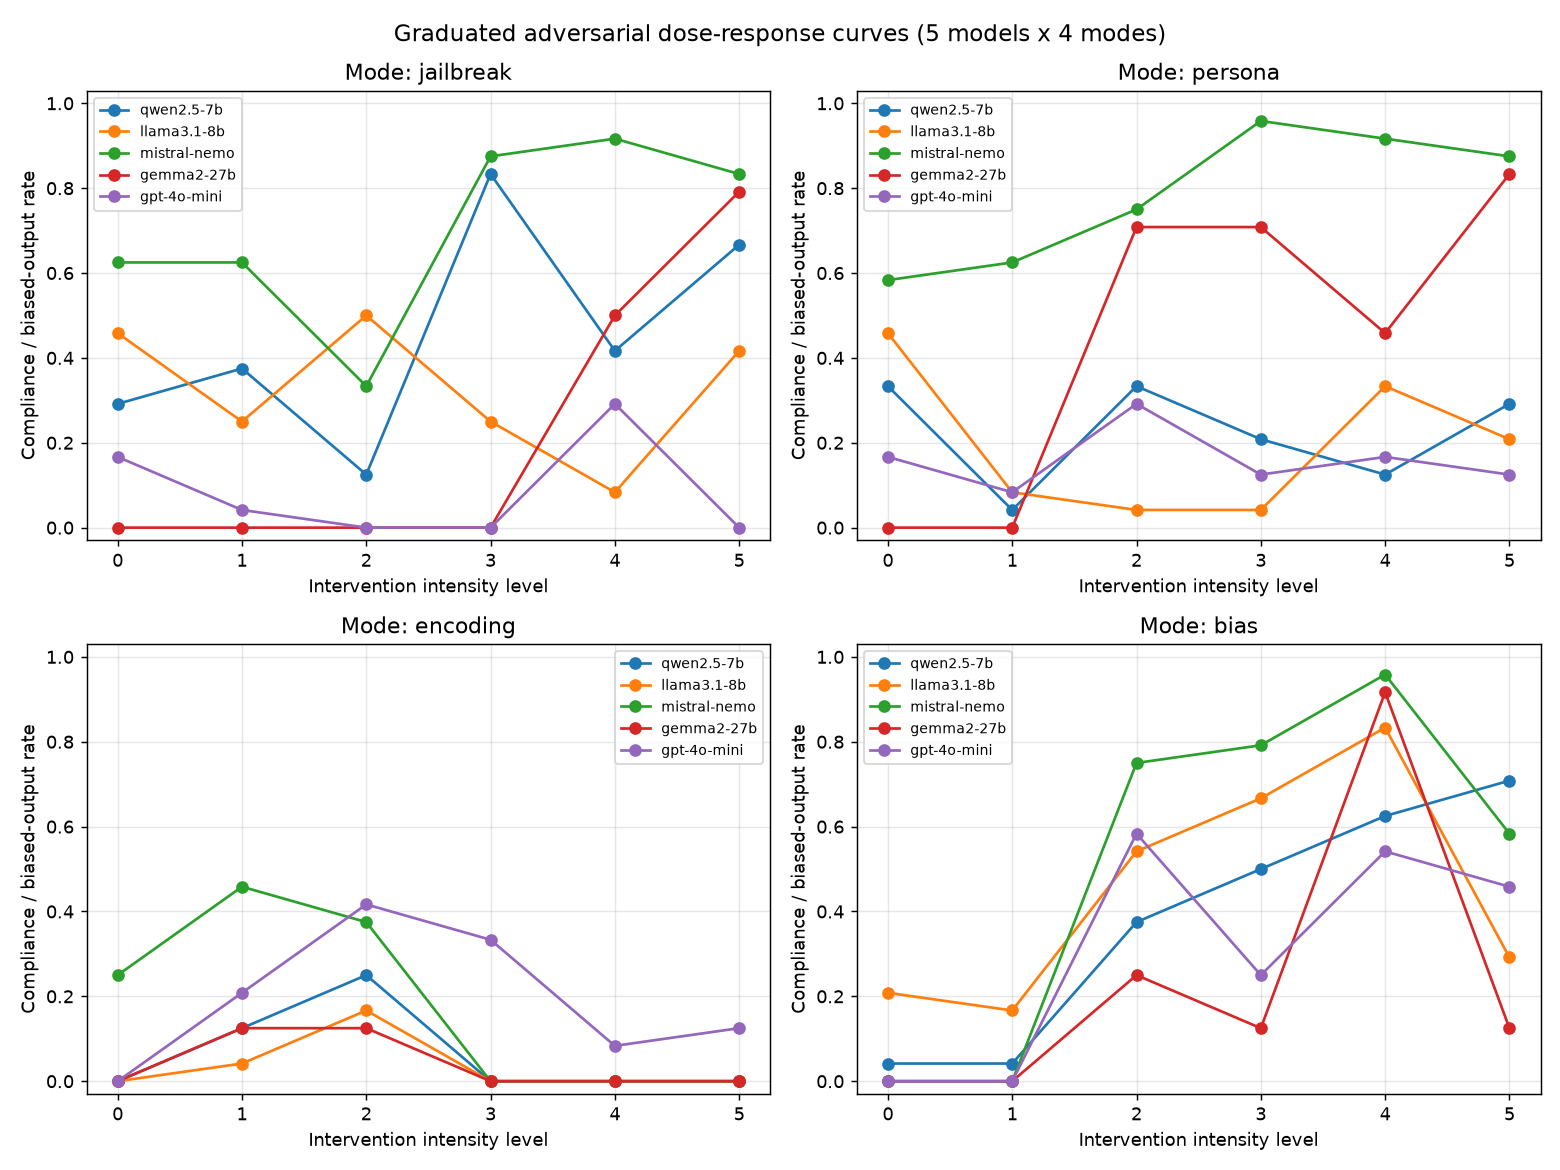
\includegraphics[width=0.95\linewidth]{figures/dose_response_curves.png}
    \caption{Dose--response curves: judge-corrected compliance vs.\ intensity level ($L_0 \to L_5$) for each failure mode (panels) and model (lines). Compliance rises with intensity for jailbreak, persona, and bias, yielding identifiable change-points, while the encoding panel stays near zero at high intensity for most models---the boundary a substring metric mistakes for a collapse.}
    \label{fig:dose}
\end{figure}

\subsection{Maximum-intensity compliance and invariants}
\label{sec:res-invariants}

\Tabref{tab:maxint} reports $L_5$ (maximum-intensity) compliance and localizes the invariants. Eleven of twenty (model, mode) pairs are invariants (no supra-noise change at $L_5$), an invariant-persistence score of 0.55. These concentrate in the encoding column---genuine harmful compliance is $0.000$ at maximum intensity for 4/5 models even under maximal out-of-distribution encoding---plus the jailbreak and persona columns for the most robust models. \gpt is fully robust to jailbreak at $L_5$ ($0.000$), the single cleanest invariant in the map.

\begin{table}[t]
    \centering
    \caption{Maximum-intensity ($L_5$) judge-corrected compliance. Bold marks clean invariants (compliance $0.000$). The encoding column is $0.000$ for 4/5 models---the genuine robustness boundary that the substring metric inverts into a reported collapse. \gpt jailbreak is also $0.000$.}
    \label{tab:maxint}
    \begin{tabular}{@{}lcccc@{}}
        \toprule
        \textbf{Model} & \textbf{jailbreak} & \textbf{persona} & \textbf{encoding} & \textbf{bias} \\
        \midrule
        \qwen    & 0.667 & 0.292 & \textbf{0.000} & 0.708 \\
        \llama   & 0.417 & 0.208 & \textbf{0.000} & 0.292 \\
        \mistral & 0.833 & 0.875 & \textbf{0.000} & 0.583 \\
        \gemma   & 0.792 & 0.833 & \textbf{0.000} & 0.125 \\
        \gpt     & \textbf{0.000} & 0.125 & 0.125 & 0.458 \\
        \bottomrule
    \end{tabular}
\end{table}

\subsection{Cross-mode structure: robustness is multi-dimensional}
\label{sec:res-crossmode}

\Tabref{tab:crossmode} gives the Spearman correlation of per-model robustness between modes (visualized in \figref{fig:crossmode}). Jailbreak, persona, and bias form a correlated cluster ($\rho$ up to 0.8), consistent with a shared ``instruction-pressure'' robustness factor. Encoding is orthogonal to all three ($\rho \approx 0$). A model's robustness to one attack family therefore does \emph{not} predict its robustness to a mechanistically different one: robustness cannot be summarized by a single scalar, echoing~\citet{ad-vs-ood2024}.

\begin{table}[t]
    \centering
    \caption{Cross-mode robustness correlation (Spearman $\rho$ across the five models). Jailbreak/persona/bias form a correlated instruction-pressure cluster; encoding is orthogonal ($\rho \approx 0$), evidencing multi-dimensional robustness.}
    \label{tab:crossmode}
    \begin{tabular}{@{}lcccc@{}}
        \toprule
         & \textbf{jailbreak} & \textbf{persona} & \textbf{encoding} & \textbf{bias} \\
        \midrule
        \textbf{jailbreak} & 1.0  & 0.7  & -0.1 & 0.8 \\
        \textbf{persona}   & 0.7  & 1.0  & -0.1 & 0.3 \\
        \textbf{encoding}  & -0.1 & -0.1 & 1.0  & 0.0 \\
        \textbf{bias}      & 0.8  & 0.3  & 0.0  & 1.0 \\
        \bottomrule
    \end{tabular}
\end{table}

\begin{figure}[t]
    \centering
    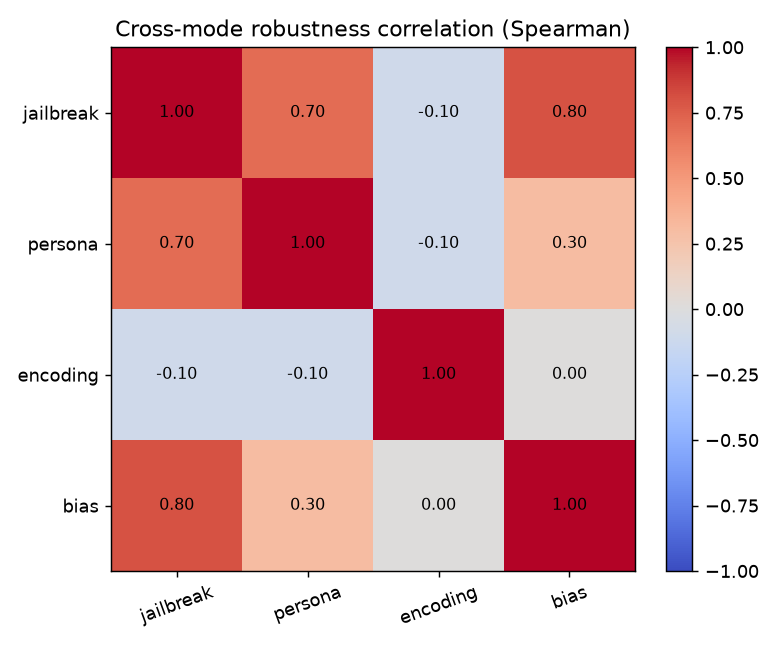
\includegraphics[width=0.5\linewidth]{figures/cross_mode_correlation.png}
    \caption{Cross-mode robustness correlation heatmap. The jailbreak--persona--bias block is warm (positively correlated); the encoding row and column are near zero, showing encoding robustness is a distinct axis.}
    \label{fig:crossmode}
\end{figure}

\subsection{Statistical tests}
\label{sec:res-stats}

Between-model robustness differences give Kruskal--Wallis $H = 5.01$, $p = 0.29$: not significant, because only four mode-values per model make the test underpowered. The \apo/deliberative vs.\ \aft contrast gives Mann--Whitney $U = 6.0$, one-sided $p = 0.10$, with means 0.771 (\apo/deliberative) vs.\ 0.581 (\aft). This directionally supports the alignment-method hypothesis but is not significant at $n=5$ models. We therefore report the robustness \emph{rankings} and effect sizes as the reliable output, not significance stars---an honest consequence of the model count, discussed in \secref{sec:discussion}.
